\documentclass{article}
\usepackage{hyperref}
\usepackage{graphicx}
\usepackage{float}
\begin{document}
	\section{ACD - Analog to Digital Conversion} % (fold)
	\label{sec:acd_analog_to_digital_conversion}
	An ACD converter is needed to translate analog data (temperature) from the thermistor to digital data (voltage) that the RaspberryPi can understand. If I were using an Arduino I would not need such a converter as an Arduino has an ADC converter built in where as the RaspberryPi is a digital only microcontroller. Using the MCP3008 for ADC, its pin out:
	\begin{itemize}
	\item VDD - power
	\item DGND - Digital ground
	\end{itemize}
	used to power the converter
	\begin{itemize}
	\item DOUT - data out of the coverter (the covnerted data we desire)
	\item CLK - clock pin
	\item DIN - data in from raspberry pi
	\item CS - Chip select
	\end{itemize}
	These 4 pins are used for the SPI (Serial Peripheral Interface) of the raspberry pi. Section \ref{sec:spi_serial_peripheral_interface} gives more on this.

	\begin{itemize}
		\item AGND - analog ground (used for precision which is optional and so can merely be connected to GND)
		\item Vref - analog reference voltage (used as a scale for the ADC)
	\end{itemize}

	Everything above comes from \href{https://learn.adafruit.com/reading-a-analog-in-and-controlling-audio-volume-with-the-raspberry-pi?view=all}{Analog Inputs for Raspberry Pi Using the MCP3008}. Discussed below is how we can use this digital data from the ADC converter to translate the data into what we expect, see \href{https://learn.sparkfun.com/tutorials/analog-to-digital-conversion/all#:~:text=An%20Analog%20to%20Digital%20Converter,pin%20to%20a%20digital%20number.&text=ADCs%20can%20vary%20greatly%20between,%5E10)%20discrete%20analog%20levels.}{Analog to Digital Conversion by Adapfruit} for more.

	Consider a microcontroller is powered with 5v, it understands 0v as a binary 0 and 5v as a binary 1. Now we have a problem when the voltage is anything between 0 and 5 volts (what will be binary 0 and what is binary 1) - this is analog data and is why micocontrollers have difficult time translating what analog data means, this is why we need an ADC converter, to understand analog data in a form it understands (digital data). The MCP3008 ADC converter is a 10-bit converter, meaning it can detect $2^{10} = 1024$ discrete analog levels. The ADC is a ratio value given as $\frac{Resolution of the ADC converter}{System Voltage} = \frac{ADC Reading}{Analog Voltage Measured}$. This means the converter will use the value 1023 to depict the system voltage and value between 0 and 1024 will be a ratio between the 5V and the ADC value 1023. The system voltage of the raspberry pi is either 3.3V or 5V dependending on the voltage pin used to power the converter. Thus we can get the \textit{analog voltage} from this equation that uses ADC values. As an example, imagine we are measuring a voltage with our Pi and the system voltage we are using is 5V, lets assume the ADC value measured on the Pi is 434 and we are using a 10-bit ADC converter. Now to get the analog voltage from this we do the following
	\begin{equation}
		\begin{array}{ccc}
			\frac{1023}{5} & = & \frac{434}{Analog Voltage Measured}\\
	 		Analog Voltage Measured & = & 2.12V
		\end{array}
	 \end{equation} 
	
	% section acd_analog_to_digital_conversion (end)

	\section{SPI - Serial Peripheral Interface} % (fold)
	\label{sec:spi_serial_peripheral_interface}
	SPI is a communication proocol. SPI is used for synchronous communucation between devices (a master and a slave). The 4 connections of SPI:
	\begin{itemize}
		\item SCLK - clock 
		\item MOSI - Master Out Slave In which is a data line from the master device to the slave device
		\item MISO - Master In Slave Out which is another data line for sending data from a slave to a master
		\item SS - Slave Select used to tell the slave that it must be on the 'look out' for data (either sending or receiving)
	\end{itemize}
	As the pins suggested, devices oeprating with SPI can act either as a slave or as a master. The SS pin also hints at the ablity to connect multiple slaves to a master device. We can have 3 slaves and we can select which one we want to communicate with (either to receive data from them or to send data to) by applying or not applying voltage to the slave's SS connectionof interest. To start communucation with a slave device we set the SS pin to low.

	\begin{figure}[H]
	\centering
	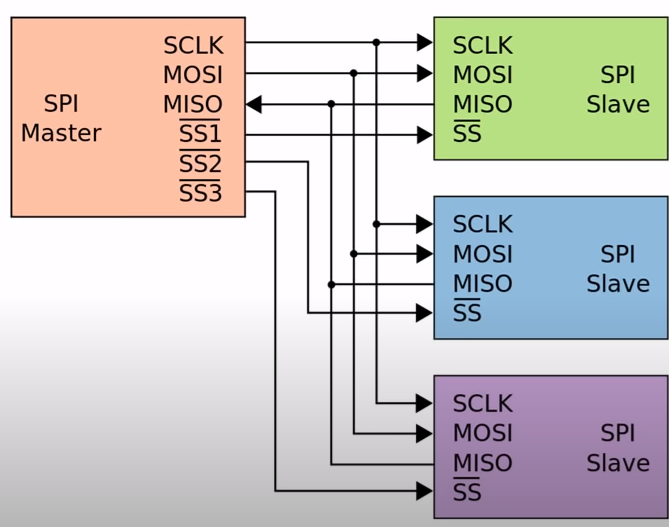
\includegraphics[width=0.5\textwidth]{images/multi_slave.png}
	\caption{Image from \href{https://www.youtube.com/watch?v=ba0SQwjTQfw}{nanland}}	
	\end{figure}

	SPI is full duplex meaining you can send and receive data at the same time. It is not suited for long distance communication (\href{https://www.youtube.com/watch?v=ba0SQwjTQfw}{nanland} goes as far as saying that even more than a meter is not suited for SPI).

	Now when it comes to programming the microcontroller for SPI communication, there are 4 modes of SPI we can set that correspond to when data must be read based on the clock signal send from master to slave via the CLK pin. These 4 modes can be 
	\begin{enumerate}
		\item Read/write when clock is low and on rising edge
		\item Read/write when clock is high and on rising edge
		\item Read/write when clock is low and on falling edge
		\item Read/write when clock is high and on rising edge
	\end{enumerate}

	\href{https://www.youtube.com/watch?v=fvOAbDMzoks&t=6s}{Great Scott} explains the modes rather well. The mode to use depends on the device being used, see the datasheet of the device for more.

	SPI transfers data at a CRAZY rate and is part in parsle the reason for its existance

	There are 2 ways we can use SPI communication, software SPI or hardware SPI. Hardware SPi is if the devei has pins built specifically for SPI communication. Software SPI is used for devices that can be programmed to use the SPI protocol.
	
	% section spi_serial_peripheral_interface (end)

	\section{Thermistor - Reading Temperature From Voltage} % (fold)
	\label{sec:thermistor_reading_temperature_from_voltage}
	An article titled \href{https://www.jameco.com/Jameco/workshop/techtip/temperature-measurement-ntc-thermistors.html#:~:text=Thermistor%20Response%20to%20Temperature,in%20response%20to%20temperature%20change.}{Thermistors/Temperature Measurement with NTC Thermistors} was referenced for this section of the research. As well as an adafruit tutorial on the matter thant can be found \href{https://learn.adafruit.com/thermistor/using-a-thermistor}{here}.

	An NTC (Negative Temperature Coefficient) thermistor will decrease its resitance with an increase in temperature.

	To measure temperature with a thermistor we need to measure the resitance of the thermistor. To do this we can measure the voltage and an additional resitor along with the voltage divider and Ohm's law to calculate the resistance - we can get a better reading by averaging values and by using voltage lines that dont have noise on them. From the resitance we can convert it to a temperature reading using the Steinhart Equation (not as accuate as a temperature table that is provided by the manufacturer of the thermistor). It is given as 
	\begin{equation}
		\frac{1}{T} = A + Bln(R) + C(ln(R))^3
	\end{equation}
	This equation can be used if the manufacturer of the thermsitor provides the values for $A, B$ and $C$. An alternative is the simplified B parameter equation that only depends on the constant $B$ which most manufacturers do provide. 
	\begin{equation}
	 	\frac{1}{T} = \frac{1}{T_0} + \frac{1}{B}ln(\frac{R}{R_0})
	 \end{equation} 
	 Where $T_0$ and $R_0$ are kelvin room temperature and resitance at room temperature. This is essentially the steinhat equation with values for $A$ and $C$ substituted for specific values (see \href{https://en.wikipedia.org/wiki/Thermistor}{Wikipedia} for more).
	
	% section thermistor_reading_temperature_from_voltage (end)

	\section{MCP3002} % (fold)
	\label{sec:mcp3002}
	The pip gpiozero package was used to read the ADC value obtained by the MCP3002 \href{https://gpiozero.readthedocs.io/en/stable/api_spi.html}{API - SPI Devices}. There simply was not code online to run the java version using pi4j and so I had to revert to this option. A number of ways exist to read and execute a python script as listed by this \href{https://www.baeldung.com/java-working-with-python}{Baeldung} tutorial. The ProcessBuilder class was the option that was opted for to execute the mcp3002\_adc\_value.py script which was also saved to the resources folder of the pump-controller project for history purposes. To read the code the following script was generated 
	\begin{figure}[H]
	\centering
	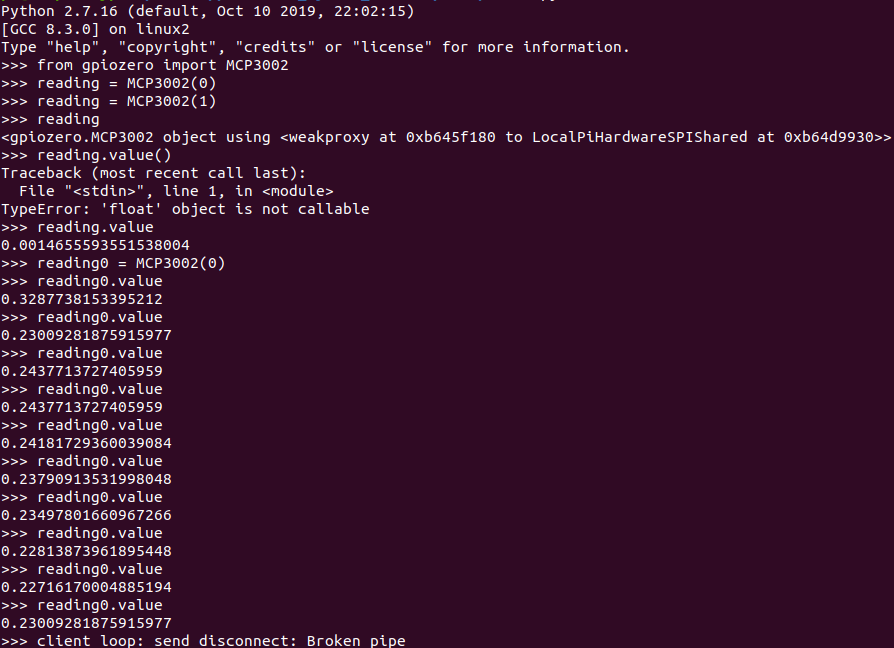
\includegraphics[width=\textwidth]{images/mcp3002_gpiozero_code_read_adc.png}
	\caption{Terminal Code :)}	
	\end{figure}


	
	% section mcp3002 (end)

	\section{MCP3002 and Thermistor Results}
	There exists a (roughly) $2.5$ degrees celsius error between the converted MCP3002 ADC obtained temperature and the true reading of the temperature.

	\section{Ground} % (fold)
	\label{sec:ground}
	The RaspberryPi grounds may have some noise on them. To check this simply connect your multimeter to the various ground points of the RaspberryPi. The voltage between the grounds must be 0. If this is not the case then its time to play the illimunation game to determine which ground gives a voltage other than 0. The culprit will be the one prone to noise. Simply use another ground on the RaspberryPi. 
	
	% section earthing (end)


\end{document}